\documentclass[letterpaper]{article}
\usepackage[margin=1in]{geometry} % Sets page size and 1-inch margins
\usepackage[svgnames,dvipsnames]{xcolor}   % svgnames is a superset of dvipsnames

\usepackage{amsmath} % For math symbols like \land, \langle, \rangle, \to
\usepackage{array}   % For advanced column specifications
\usepackage{tabularx}% For tables with auto-expanding columns
\usepackage{tikz}
\usetikzlibrary{
    positioning,      % For placing nodes relative to each other (e.g., below=of)
    shapes.geometric, % For shapes like ellipses
    arrows.meta,      % For advanced arrow tips (e.g., Stealth)
    decorations.pathmorphing, % For snake/squiggly lines
    calc              % For coordinate calculations
}

% --- GLOBAL STYLE DEFINITIONS FOR DFD ---
\tikzset{
    % A shape for logical connectives
    connective_node/.style={
        rectangle, rounded corners=5pt, draw=black!80, fill=black!10, 
        inner sep=5pt, thick, align=center
    },
    % A shape for Introduction Rules
    intro_rule_node/.style={
        rectangle, rounded corners=5pt, draw=black!80, fill=Teal!20, 
        inner sep=5pt, thick, align=center
    },
    % A shape for Elimination Rules
    elim_rule_node/.style={
        rectangle, rounded corners=5pt, draw=black!80, fill=BurntOrange!20, 
        inner sep=5pt, thick, align=center
    },
    % A shape for abstract propositions
    proposition_node/.style={
        ellipse, draw=black!80, fill=Violet!15,
        inner sep=3pt, align=center
    },
    % A shape for concrete proof terms
    proof_node/.style={
        ellipse, draw=black!80, fill=Green!15,
        inner sep=3pt, align=center
    },
    % Interface ports for composition
    input_port/.style={
        circle, draw=blue!70!black, fill=blue!20,
        inner sep=2pt, minimum size=8pt
    },
    output_port/.style={
        circle, draw=ForestGreen!80!black, fill=ForestGreen!20,
        inner sep=2pt, minimum size=8pt
    },
    % Arrow styles with color
    input_arrow/.style={-Stealth, solid, thick, draw=blue!70!black},
    output_arrow/.style={double, double distance=1.5pt, -Stealth, solid, thick, draw=ForestGreen!80!black},
    proves_arrow/.style={-Stealth, decorate, decoration={snake, segment length=6pt, amplitude=1pt}, thick, draw=orange!90!black}
}

% --- Define and measure boxes to get widths for tabularx ---
\newlength{\andheaderwidth}
\settowidth{\andheaderwidth}{\textbf{And} : Prop $\to$ Prop $\to$ Prop}
\newlength{\andintrofooterwidth}
\settowidth{\andintrofooterwidth}{\textbf{And.intro} : P $\to$ Q $\to$ P $\land$ Q}

\begin{document}

\begin{figure}[h!]
\centering
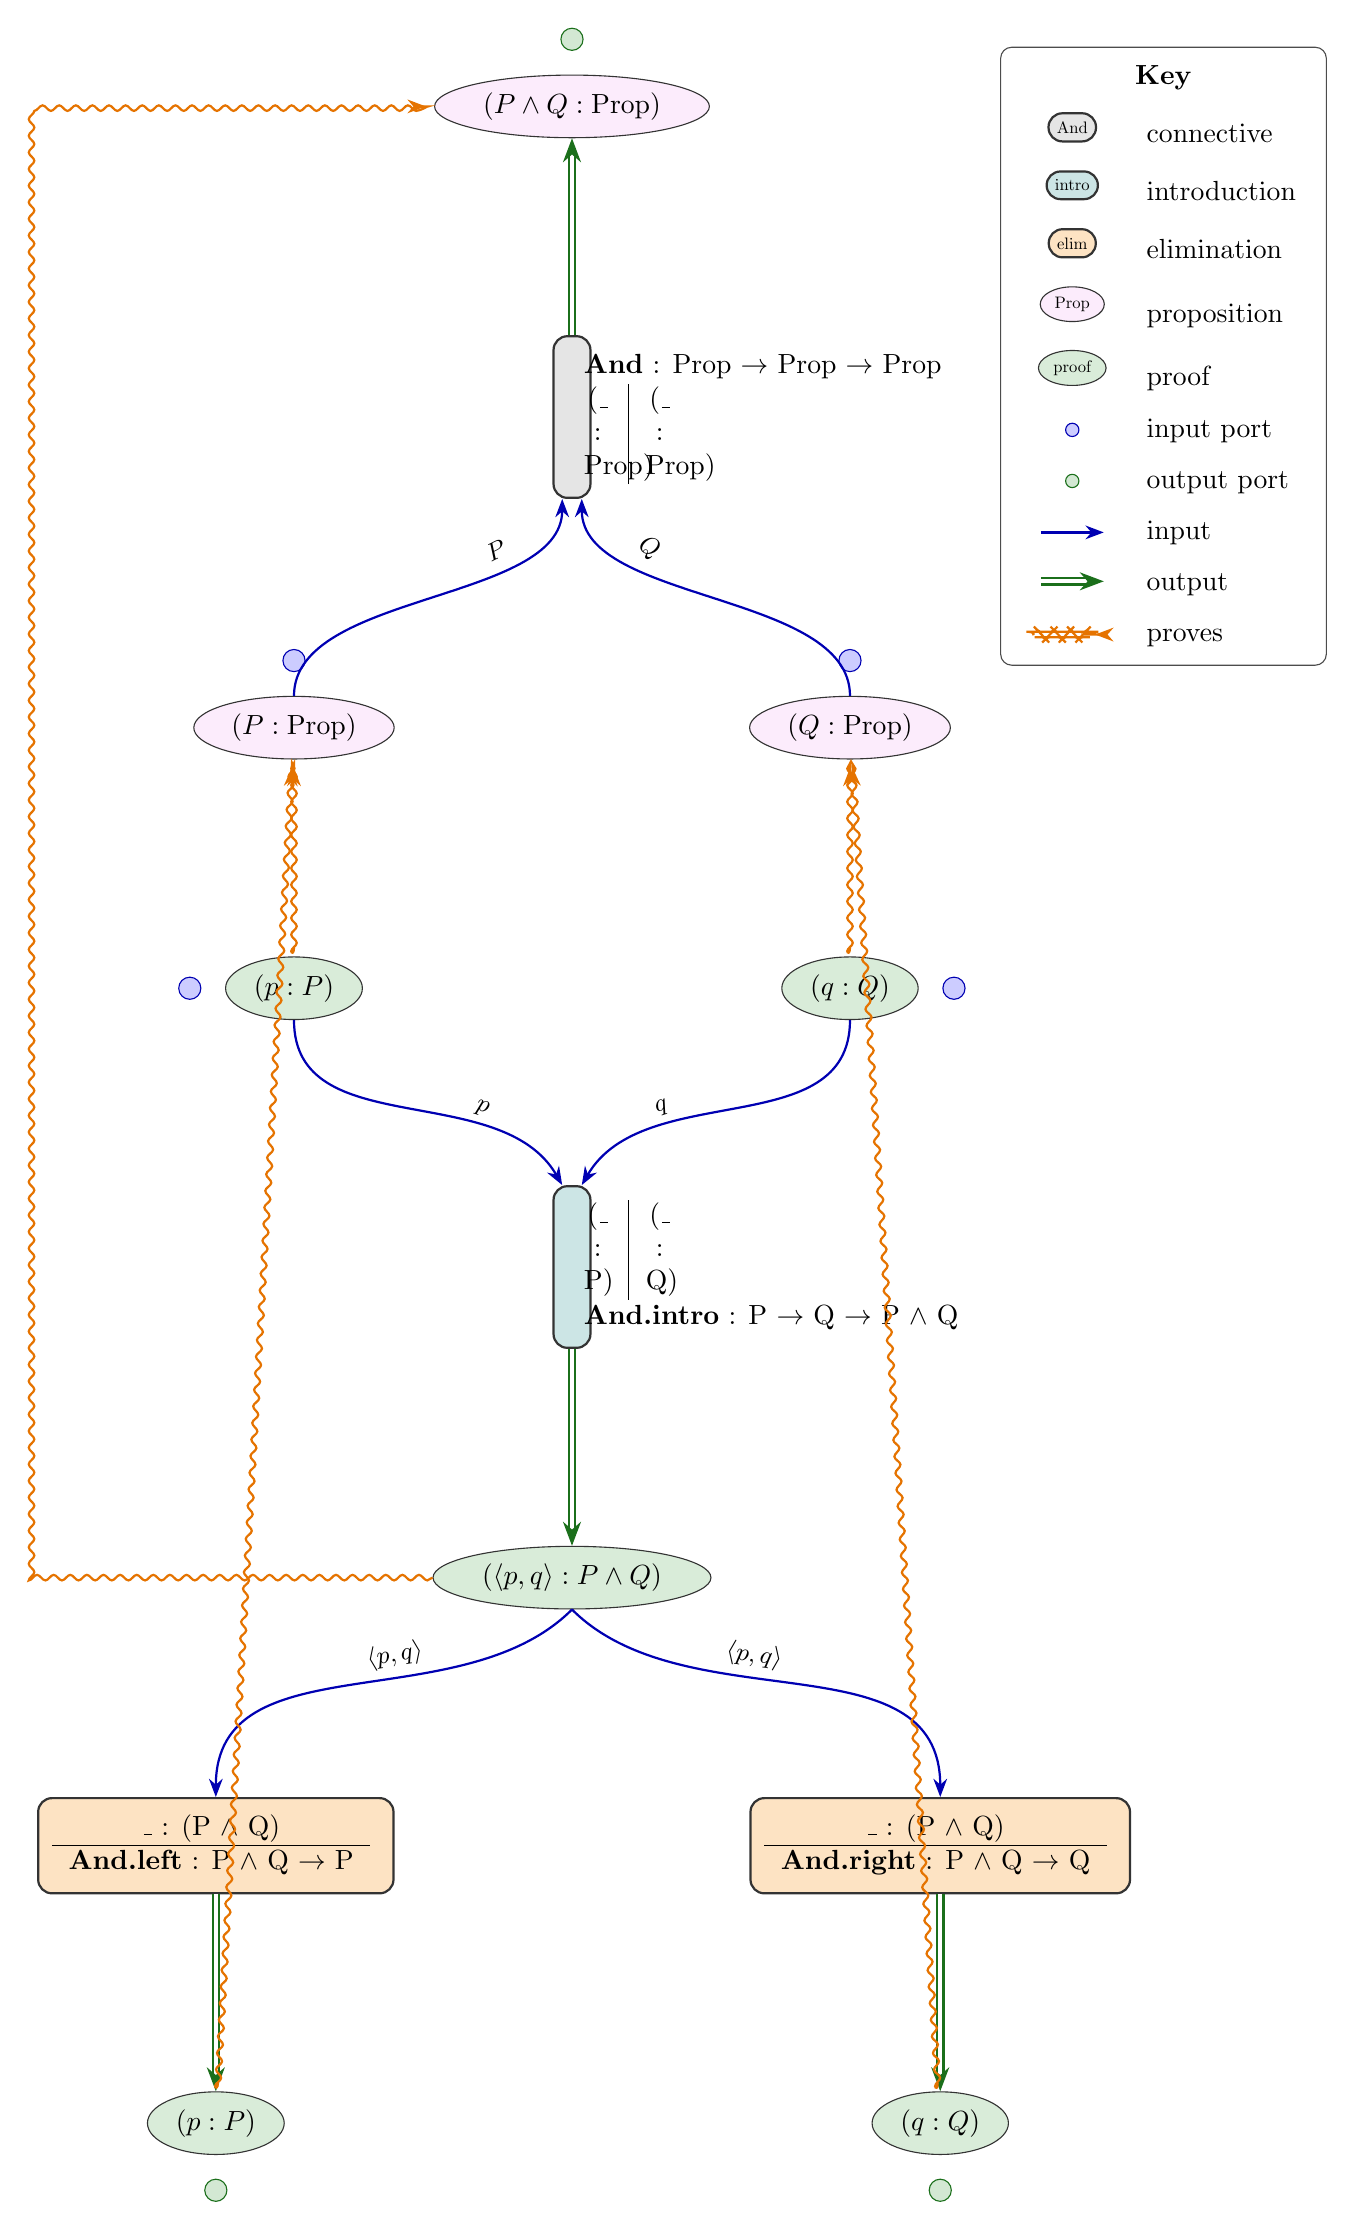
\begin{tikzpicture}[node distance=2.5cm and 2.5cm]

% --- INPUT TYPE PARAMETERS ---
\node[proposition_node] (P_prop) {$(P : \text{Prop})$};
\node[proposition_node] (Q_prop) [right=4.5cm of P_prop] {$(Q : \text{Prop})$};

% Input ports for type parameters
\node[input_port] (P_in_port) [above=0.3cm of P_prop] {};
\node[input_port] (Q_in_port) [above=0.3cm of Q_prop] {};

% --- CONNECTIVE LAYER ---
\node[connective_node, above=2.5cm of $(P_prop.north)!.5!(Q_prop.north)$] (and_box) {
    \begin{tabularx}{\andheaderwidth}{>{\centering\arraybackslash}X|>{\centering\arraybackslash}X}
        \multicolumn{2}{c}{\textbf{And} : Prop $\to$ Prop $\to$ Prop} \\ \hline
        (\_ : Prop) & (\_ : Prop)
    \end{tabularx}
};

\node[proposition_node] (P_and_Q_prop) [above=2.5cm of and_box] {$(P \land Q : \text{Prop})$};

% Output port for result type
\node[output_port] (type_out_port) [above=0.3cm of P_and_Q_prop] {};

% --- INTRODUCTION SECTION ---
% Input proof ports
\node[proof_node] (p_P) [below=2.5cm of P_prop] {$(p : P)$};
\node[proof_node] (q_Q) [below=2.5cm of Q_prop] {$(q : Q)$};
\node[input_port] (p_in_port) [left=0.3cm of p_P] {};
\node[input_port] (q_in_port) [right=0.3cm of q_Q] {};

% Introduction rule
\node[intro_rule_node, below=2.5cm of $(p_P)!.5!(q_Q)$] (and_intro) {
    \begin{tabularx}{\andintrofooterwidth}{>{\centering\arraybackslash}X|>{\centering\arraybackslash}X}
    (\_ : P) & (\_ : Q) \\ \hline
    \multicolumn{2}{c}{\textbf{And.intro} : P $\to$ Q $\to$ P $\land$ Q}
    \end{tabularx}
};

\node[proof_node] (pq_pair) [below=2.5cm of and_intro] {$(\langle p, q \rangle : P \land Q)$};

% --- ELIMINATION SECTION ---
% Elimination rules
\node[elim_rule_node, below left=2.5cm and 1cm of pq_pair] (and_left) {
    \begin{tabular}{c}
    \_ : (P $\land$ Q) \\ \hline
    \textbf{And.left} : P $\land$ Q $\to$ P
    \end{tabular}
};

\node[elim_rule_node, below right=2.5cm and 1cm of pq_pair] (and_right) {
    \begin{tabular}{c}
    \_ : (P $\land$ Q) \\ \hline
    \textbf{And.right} : P $\land$ Q $\to$ Q
    \end{tabular}
};

% Output proof ports
\node[proof_node] (result_p) [below=2.5cm of and_left] {$(p : P)$};
\node[proof_node] (result_q) [below=2.5cm of and_right] {$(q : Q)$};
\node[output_port] (p_out_port) [below=0.3cm of result_p] {};
\node[output_port] (q_out_port) [below=0.3cm of result_q] {};

% --- EDGE ROUTING ---
\draw[output_arrow] (and_box) -> (P_and_Q_prop);
\draw[input_arrow] (P_prop.north) to[out=90, in=-90, looseness=0.8] node[pos=0.7, sloped, above, font=\small] {$P$} ($(and_box.south west)!.5!(and_box.south)$);
\draw[input_arrow] (Q_prop.north) to[out=90, in=-90, looseness=0.8] node[pos=0.7, sloped, above, font=\small] {$Q$} ($(and_box.south)!.5!(and_box.south east)$);

\draw[input_arrow] (p_P.south) to[out=-90, in=120] node[pos=0.7, sloped, above, font=\small] {$p$} ($(and_intro.north west)!.5!(and_intro.north)$);
\draw[input_arrow] (q_Q.south) to[out=-90, in=60] node[pos=0.7, sloped, above, font=\small] {$q$} ($(and_intro.north)!.5!(and_intro.north east)$);

\draw[output_arrow] (and_intro) -> (pq_pair);

\draw[input_arrow] (pq_pair.south) to[out=-135, in=90] node[pos=0.4, sloped, above, font=\small] {$\langle p, q \rangle$} (and_left.north);
\draw[input_arrow] (pq_pair.south) to[out=-45, in=90] node[pos=0.4, sloped, above, font=\small] {$\langle p, q \rangle$} (and_right.north);

\draw[output_arrow] (and_left) -> (result_p);
\draw[output_arrow] (and_right) -> (result_q);

% Proves arrows
\draw[proves_arrow, shorten <=3pt, shorten >=3pt] (p_P) -> (P_prop);
\draw[proves_arrow, shorten <=3pt, shorten >=3pt] (q_Q) -> (Q_prop);
\draw[proves_arrow, shorten <=3pt, shorten >=3pt] (result_p) -> (P_prop);
\draw[proves_arrow, shorten <=3pt, shorten >=3pt] (result_q) -> (Q_prop);

% Main "proves" arc
\coordinate (outset_point) at ($(P_prop.west)+(-2cm,0)$);
\draw[proves_arrow, shorten >=3pt] (pq_pair.west) -- (outset_point |- pq_pair.west) -- (outset_point |- P_and_Q_prop.west) -- (P_and_Q_prop.west);

% --- LEGEND ---
\node (legend) [draw=black!70, rounded corners, inner sep=5pt, above right=0.5cm and 1cm of Q_prop] {
    \begin{tabular}{cl}
    \multicolumn{2}{c}{\textbf{Key}} \\[1.5ex]
    \tikz{\node[connective_node, scale=0.6] {And};} & connective \\[1.5ex]
    \tikz{\node[intro_rule_node, scale=0.6] {intro};} & introduction \\[1.5ex]
    \tikz{\node[elim_rule_node, scale=0.6] {elim};} & elimination \\[1.5ex]
    \tikz{\node[proposition_node, scale=0.6] {Prop};} & proposition \\[1.5ex]
    \tikz{\node[proof_node, scale=0.6] {proof};} & proof \\[1.5ex]
    \tikz{\node[input_port, scale=0.6] {};} & input port \\[1.5ex]
    \tikz{\node[output_port, scale=0.6] {};} & output port \\[1.5ex]
    \tikz{\draw[input_arrow] (0,0.1) -- (0.8,0.1);} & input \\[1.5ex]
    \tikz{\draw[output_arrow] (0,0.1) -- (0.8,0.1);} & output \\[1.5ex]
    \tikz{\draw[proves_arrow] (0,0.1) -- (0.8,0.1);} & proves \\
    \end{tabular}
};

\end{tikzpicture}
\caption{Modular And connective with composition interfaces. Input ports (blue) accept type parameters and proof terms. Output ports (green) provide the constructed type and proof terms for use in larger compositions. The standardized 2.5cm spacing and port system enable systematic composition with other logical operators.}
\label{fig:and_modular}
\end{figure}

\end{document}